\normaltrue \difficilefalse \tdifficilefalse
\correctionfalse

%\UPSTIidClasse{11} % 11 sup, 12 spé
%\renewcommand{\UPSTIidClasse}{12}

\exer{Train simple $\star$ \label{C2:06:21}}

\UPSTIcompetence[2]{A3-05}
\UPSTIcompetence[2]{C2-06}
\index{Compétence C2-06}
\index{Train d'engrenages simple}
\ifcorrection
\else
\marginnote{\textbf{Pas de corrigé pour cet exercice.}}
\fi

\ifprof
\else
Soit le système de transmission suivant. 
\begin{center}
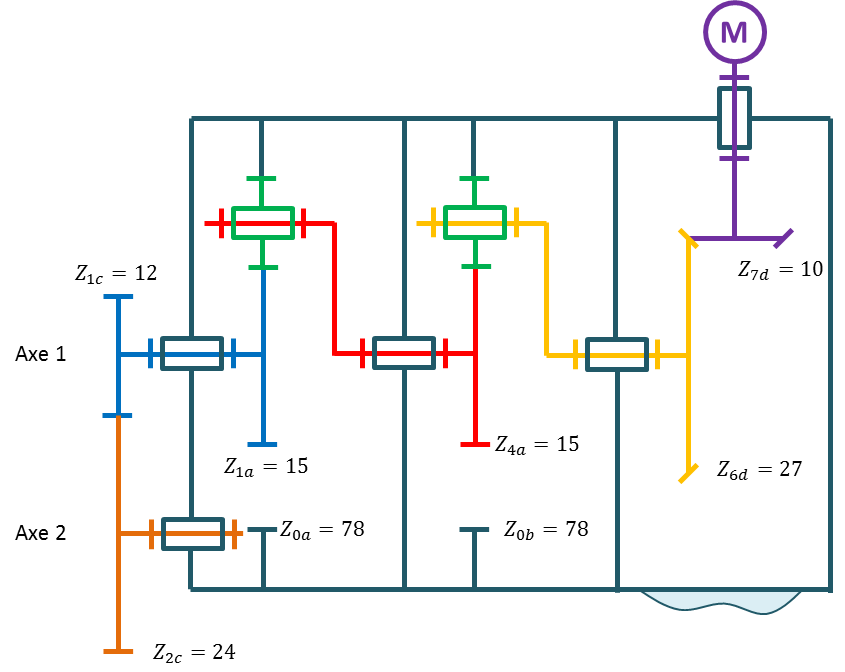
\includegraphics[width=.7\linewidth]{32_01}
\end{center}
\fi


\question{Donner les rapports de chacun des 4 étages de réduction.}
\ifprof
\else
\fi

\ifprof
\else
\begin{flushright}
\footnotesize{Corrigé  voir \ref{C2:06:21}.}
\end{flushright}%
\fi